\section{Beyond Standard Model physics}
The autoencoder is model independent to try to detect New Physics as unbiased as possible. This is because there are 
numerous amounts of possible New Physics signals that could exist in nature. To test the autoencoder two 
signals from supersymmetry were used.
\subsection*{Supersymmetry}
Supersymmetry is another Beyond Standard Model theory that attempts to solve two other problems that the SM has. 
First we have the hierarchy problem. As the SM is a perturbative theory, the Higgs mass increases at 
higher energies. The problem is that when you approach higher and higher energies, the Higgs mass goes to infinity, 
which is not physical. Supersymmetry solves this problem by introducing a supersymmetric partner to each particle
in the SM. The result is that the contributions to the Higgs mass from fermions and bosons mainly cancel each other out, 
thus fixing the hierarchy problem. Another problem we have with the SM
is that is does not have a field for dark matter, whereas some supersymmetry models have a dark matter candidate.
As supersymmetry in theory could solve some problems with the SM it is a topic of great interest with both theoretical and 
experimental physicists. Still, after three LHC runs supersymmetry has not been observed\cite{atlas_search_2021}. \par 

To test the autoencoders, two signal models from SUSY were picked. The chosen signal samples have a final state with 3 leptons + $e_T^{miss}$,
as the background does. The signal final state is shown below in figure \ref{fig:sysy_feyn}. 

\begin{figure}[H]
    \centering
    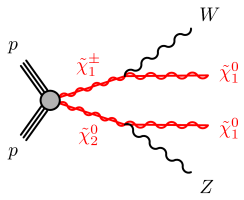
\includegraphics[width=0.4\linewidth]{Figures/susy/C1N2-WZN1N1.png}
    \caption[SUSY feynman diagram]{SUSY diagram showing chargino-neutralino prodiction in proton-proton collision. }
    \label{fig:sysy_feyn}
\end{figure}

Figure \ref{fig:sysy_feyn} shows chargino$(\tilde{\chi}_1^{\pm})$-neutralino$(\tilde{\chi}_1^{0})$ production via proton-proton collisions. 
This is a minimal supersymmetric standard model (MSSM). The chargino is the supersymmetric partner 
to the charged bosons and the neutralino is the supersymmetric partner of the neutral bosons. The neutralino
is the lightest and stable supersymmetric particle, and is therefor a good candidate for dark matter. 
The search for these particles were similarly done by ATLAS in 2021\cite{atlas_search_2021}. 